\documentclass[a4paper,10pt]{article}
%\documentclass[a4paper,10pt]{scrartcl}
\usepackage[top=3cm, bottom=3cm, left=2cm, right=2cm]{geometry}

\usepackage[utf8]{inputenc}
\usepackage[frenchb]{babel}
\usepackage{xspace}
\usepackage{listings}
\usepackage{graphicx}
\usepackage{caption}

\usepackage[T1]{fontenc}
\usepackage{Alegreya} %% Option 'black' gives heavier bold face 
\renewcommand*\oldstylenums[1]{{\AlegreyaOsF #1}}

\usepackage{bera}% optional: just to have a nice mono-spaced font
\usepackage{listings}
\usepackage{xcolor}

\colorlet{punct}{red!60!black}
\definecolor{background}{HTML}{EEEEEE}
\definecolor{delim}{RGB}{20,105,176}
\colorlet{numb}{magenta!60!black}

\lstdefinelanguage{json}{
    basicstyle=\normalfont\ttfamily,
    numbers=left,
    numberstyle=\scriptsize,
    stepnumber=1,
    numbersep=8pt,
    showstringspaces=false,
    breaklines=true,
    frame=lines,
    backgroundcolor=\color{background},
    literate=
     *{0}{{{\color{numb}0}}}{1}
      {1}{{{\color{numb}1}}}{1}
      {2}{{{\color{numb}2}}}{1}
      {3}{{{\color{numb}3}}}{1}
      {4}{{{\color{numb}4}}}{1}
      {5}{{{\color{numb}5}}}{1}
      {6}{{{\color{numb}6}}}{1}
      {7}{{{\color{numb}7}}}{1}
      {8}{{{\color{numb}8}}}{1}
      {9}{{{\color{numb}9}}}{1}
      {:}{{{\color{punct}{:}}}}{1}
      {,}{{{\color{punct}{,}}}}{1}
      {\{}{{{\color{delim}{\{}}}}{1}
      {\}}{{{\color{delim}{\}}}}}{1}
      {[}{{{\color{delim}{[}}}}{1}
      {]}{{{\color{delim}{]}}}}{1},
}




\usepackage{fancyhdr}
\pagestyle{fancy}

\renewcommand{\headrulewidth}{1pt}
\fancyhead[C]{} 
\fancyhead[L]{\leftmark}
\fancyhead[R]{Vincent Stébé}

\renewcommand{\footrulewidth}{1pt}
\fancyfoot[C]{\textbf{\thepage}} 
\fancyfoot[L]{}
\fancyfoot[R]{}

\title{Système à particules}
\author{Vincent Stébé}
\date{}


\lstset{basicstyle=\small}

\begin{document}
\maketitle

\tableofcontents
\newpage
\section{Introduction}
L'objectif est de concevoir une application interactive affichant différents effets de système à particules.
Ces effets doivent pouvoir être chargées depuis un fichier externe.
J'ai donc choisi d'orienter l'application vers un réel éditeur d'effets.
L'utilisateur peut alors créer de nouveaux effets et tester sa configuration en temps réel.

\section{Principe de fonctionnement}
\subsection{CPU ou GPU ?}
L'application peut être conçue de deux manières : soit on utilise au maximum les shaders qui vont à la fois gérer l'affichage mais aussi la physique des particules,
soit délègue la physique au CPU. Les GPU étant toujours plus efficaces, il est intéressant d'utiliser la première méthode si l'on souhaite maximiser les performances.
La gestion de la physique via le GPU nécessite l'utilisation du \emph{Transform Feedback}.
Cette fonctionnalité permet aux shaders d'éditer des variables et de les réutiliser plus tard.
\emph{Transform Feedback} est disponible depuis \emph{OpenGL 3.0} mais ne dispose de fonctions avancées qu'à partir d'\emph{OpenGL 4.0.}.
Mon ordinateur ne disposant pas de cette version d'OpenGL, j'ai choisi d'utiliser le CPU pour la gestion de la physique.
Malgré une possible mais légère perte de performances, cela me permet une très grande liberté d'effets.


\subsection{Performances}
Le CPU modifie en permanence la position des particules mais également d'autres paramètres d'affichage comme la couleur.
Il est indispensable de mettre à jour rapidement ces données.
J'ai donc utilisé le mode \emph{stream} d'édition des VBO qui accroit considérablement les performances.
On utilisera également au maximum les shaders pour l'affichage et notamment pour les rotations qui sont coûteuses.

\subsection{Configuration}
L'utilisateur doit pouvoir créer ses propres effets sans se préoccuper de la gestion de la physique ou spécifier des formules mathématiques.
On veut par exempler indiquer un vent vers la droite sans avoir à recalculer soi-même les vecteurs de vitesse et de position.
On reste donc déclaratif : l'utilisateur peut indiquer plusieurs paramètres qui seront utilisés par le système à particules.
L'utilisation d'un fichier JSON permet de garder un format simple et lisible.
\subsubsection{Les paramètres obligatoires}
Certains paramètres sont obligatoires absoluments nécessaires :
\begin{itemize}
 \item Le nombre maximum de particules \emph{(max-particles)} : les buffers ont une taille fixe, ce nombre ne pourra pas être dépassé.
 Cela permet également au système à particules de ne <<pas s'emballer>> et de garder des performances correctes.
 \item Le temps de création d'une particule \emph{(creation-time)}
 \item Le temps de vie d'une particule \emph{(life-time)}
\end{itemize}


\subsubsection{Les paramètres facultatifs}
Dans le cas où l'utilisateur ne spécifie pas ces paramètres, ils seront soit ignorés soit auront une valeur par défaut.
\begin{itemize}
 \item Les forces statiques \emph{(forces)} : il s'agit d'une liste de vecteurs fixes qui peuvent par exemple correspondre à un vent, une gravité...
 \item Une force dynamique d'attraction \emph{(attract-point)} : un point où les particules seront attirés. On spécifie également la norme de cette force d'attraction.
 \item La vitesse initiale \emph{(initial speed)} : soit un vecteur de vitesse fixe, soit un intervalle où le vecteur vitesse sera généré aléatoirement
 \item Une couleur \emph{(color)} : cela peut également être un intervalle où la couleur de la particule sera générée aléatoirement.
 \item La taille \emph{(size / death-size)} : elle peut être également générée aléatoirement à partir d'un intervalle.
 L'utilisateur peut également spécifier une taille de fin : la taille de la particule augmentera alors ou rétrécira linéairement en fonction du temps.
 \item La vitesse de rotation \emph{(rotation-velocity)}
\end{itemize}

\subsubsection{Exemple}
Le fichier JSON suivant défini un système de brouillard :
\begin{lstlisting}[language=json,firstnumber=1]
{
    "size": {"min":0.2, "max":0.6},
    "image": "data/fog.png",
    "initial-speed": {
        "x":{"min":-0.01, "max":0.01},
        "y":{"min":-0.01, "max":0.01},
        "z":{"min":-0.01, "max":0.01}
    },
    "life-time": 20,
    "max-particles": 1000,
    "creation-time": 0.5,
    "rotation-velocity": 0.5,
    "color": {
        "r":{"min":0, "max":1},
        "g":{"min":0, "max":1},
        "b":{"min":0, "max":1}
    }
}
\end{lstlisting}
Les particules ne sont soumises à aucune force, vivent longtemps (20 secondes) et de couleur aléatoire.
Elles tournent sur elle-mêmes.


\subsubsection{Parsing}
L'application dispose d'une classe \emph{ParticleConfiguration} qui contient tous ces paramètres.
Le parsing est effectué grâce à Qt qui fournit des classes \emph{QJsonObject}.

\subsection{Fenêtrage}
Il est bien plus pratique pour l'utilisateur de pouvoir modifier les paramètres du système de particules en temps-réel.
L'application dispose donc d'une interface Qt qui affiche le fichier JSON utilisé, et permet les modifications.
On peut également changer directement d'effet en ouvrant un autre fichier JSON.
La barre d'outils permet d'afficher ou non le ciel et le sol, de définir le nombre d'émetteurs et permet à l'utilisateur de choisir entre trois actions lorsqu'il bouge la souris :
\begin{itemize}
 \item Déplacement de l'émetteur
 \item Déplacement de la caméra
 \item Déplacement du point d'attraction
\end{itemize}


\section{Gestion de la physique}
\subsection{Forces en jeu}
Il faut dans un premier temps calculer la force totale appliquée à chaque particule.
On distingue deux types de forces : celles statiques et globales et la force d'attraction, qui dépend de la position du point d'attraction et du point de la particule.

\begin{center}
 \includegraphics[width=5cm]{img/forces.eps}
\end{center}
\begin{center}
 $G$ : point d'attraction \hspace{3cm} $A$ : particule
\end{center}


Sur le shéma ci-dessus, on a en bleu les forces statiques, en vert la force d'attraction et en noir la force totale exercée sur la particule.
$$\vec{F} = \vec{A} + \vec{G} + \vec{V}$$

\paragraph{Force d'attraction} : dans cet exemple, sa norme est de 1.
Il est cependant possible d'utiliser un autre calcul de la norme, qui dépend de la distance entre la particule et le point d'attraction :
$|\vec{A}|=\frac{1}{d(A,G)^2}$
Ce mode de calcul permet de nouveaux types d'effets.
\subsection{Accélération}
Il s'agit en fait d'implémenter les notions de physique de base de Newton.
On a de façon générale :
$$\vec{a}m = \sum\vec{F}_{ext}$$
Avec l'accélération $\vec{a}$, la masse $m$ et les forces $\vec{F}$.
Notons que toutes les particules ont la même masse que l'on peut mettre à 1.
Il suffit de mettre à jour la position de la particule $\vec{P}$ en fonction du temps $t$ écoulé depuis la dernière mise à jour :
$$\vec{P} := \vec{P} + t \vec{a}$$
\section{Les effets}
\subsection{Feu}
\subsection{Fumée}
\subsection{Brouillard}
\subsection{Atome}

\section{Améliorations possibles}
Cette application n'est qu'une ébauche d'un projet qui pourrait être bien plus grand.
Voici quelques idées d'améliorations :
\begin{itemize}
 \item Véritable interface de contrôle du système à particules : actuellement, la configuration se fait par fichier JSON.
 L'utilisateur peut certes l'éditer en temps-réel, mais une interface à base de sliders et de sélecteurs pour chaque paramètre pourrait permettre d'ouvrir l'application à un peu large public.
 L'utilisation serait alors bien plus ludique.
 \item De nouveaux effets : sans forcément étendre le nombre de paramètres possibles, il est possible d'ajouter de nouveaux effets sympatiques.
 On pourrait créer des effets de pluie, d'éruptions, de phénomènes astronomiques... en ajoutant simplement de nouveaux fichiers JSON.
 \item Une configuration plus avancée : on peut par exemple imaginer l'intégration de formule mathématiques dans le fichier JSON.
 L'idée serait de pouvoir utiliser sans recompiler d'autres formes de distributions aléatoires ou encore d'autres formules décrivant la norme des forces.
 \item Mixer les systèmes à particules : actuellement, on peut placer plusieurs émetteurs sur la scène mais correspondant uniquement à la même configuration.
 Il faudrait pouvoir placer par exemple le feu et la fumer en même temps.
\end{itemize}


\section{Conclusion}

\end{document}
